\documentclass{article}
\usepackage[utf8]{inputenc}
\usepackage{geometry}
\usepackage{url}
\usepackage[utopia]{mathdesign}
 \geometry{
 a4paper,
 total={170mm,257mm},
 left=20mm,
 top=20mm,
 }
 \usepackage{graphicx}
 \usepackage{titling}

 \title{A brief review of a jellyfish-like soft robot
}
\author{GU JUN}
\date{September 30. 2024}
 
 \usepackage{fancyhdr}
\fancypagestyle{plain}{%  the preset of fancyhdr 
    \fancyhf{} % clear all header and footer fields
    \fancyfoot[R]{
\includegraphics[width=5cm]{science_of_soft_robot.png}}
    \fancyfoot[L]{\thedate}
    \fancyhead[L]{Soft Robotics Home Assignment \#1}
    \fancyhead[R]{\theauthor}
}
\makeatletter
\def\@maketitle{%
  \newpage
  \null
  \vskip 1em%
  \begin{center}%
  \let \footnote \thanks
    {\LARGE \@title \par}%
    \vskip 1em%
    %{\large \@date}%
  \end{center}%
  \par
  \vskip 1em}
\makeatother

\usepackage{lipsum}  
\usepackage{cmbright}

\begin{document}

\maketitle

\noindent\begin{tabular}{@{}ll}
    Student & \theauthor\\
    Paper Title & SoJel –A 3D printed jellyfish-like robot using soft materials for
underwater applications \\
    Institute name & Humanoid, Biorobotics and Smart Systems Laboratory, The University of Texas at Dallas \\
    Institute web URL & \url{https://personal.utdallas.edu/~yonas.tadesse/} \\
\end{tabular}
% working principle, advantage, novelty, and what interests you.

\section*{Working Principle}
 SoJel, is a 3D printed bio-mimetic soft jellyfish robot with flexible TPU material that uses NiTi Flexinol\,\textsuperscript{\tiny\textregistered} spring actuators as artificial muscles. It has flexible 3D printed sensors at the bell margin and an energy harvesting system that is integrated for harvesting wave motion as electricity. The robot does not require the assembly of different components, except the artificial muscles and pulleys. A 406-mm-diameter molded silicone skirt (for energy harvesting and sensor) is integrated on top of the 3D printed structure to mimic the motion behavior of a real jellyfish.

\begin{figure}
    \centering
    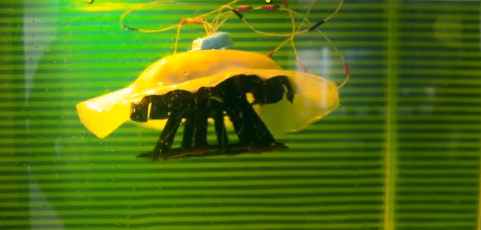
\includegraphics[width=0.6\linewidth]{jellyfish_robot.png}
    \caption{SoJel, the jellyfish-like robot, is swimming}
    \label{fig:enter-label}
\end{figure}

\section*{Advantage}
1. Most of the body is 3D printed, so the robot is easy to assemble.\\
2. TPU material spring actuators enable the robot acting as a real jellyfish.\\
3. Harvesting wave motion system allows the robot collects energy from the environment.\\
\section*{Novelty}
1. A mesoscale size soft jellyfish robot (300 mm–1 m in diameter) that can be 3D printed. \\
2. Many researches about real jellyfishes are reproduced and compared with the robot.\\
3. Sensors are 3D printed and specially designed for the robot.\\

\section*{What Interests Me}
1. This is a jellyfish-like soft robot that highly mimics the real jellyfishes' motion.\\
2. The robot has an energy harvesting system that enables the robot can produce energy.\\
3. The most of the robot including sensors are 3D printed.\\
\end{document}
